\begin{figure*}
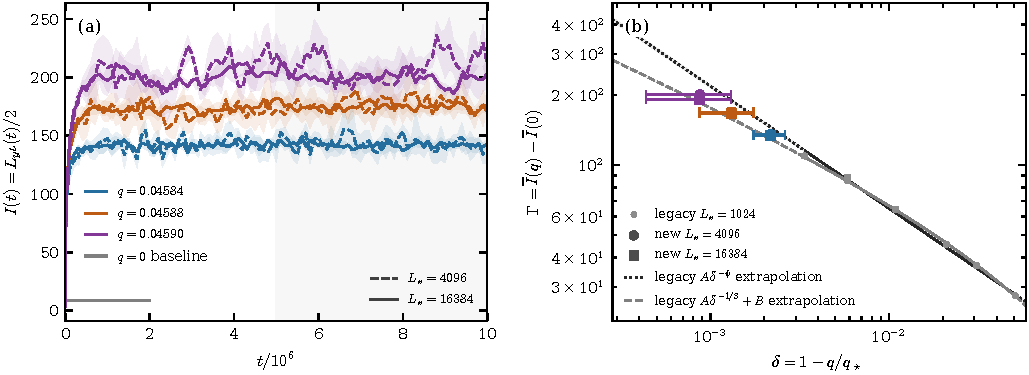
\includegraphics[width=\textwidth]{figs/fig_gpu_wetting}
\caption{Extended wall trajectories at $p=\alpha=1/2$, $L_y=8192$,
and $L_x=4096$ or 16384. Each nonzero-$q$ group contains four independent
runs to $10^7$ steps; each matching $q=0$ baseline contains two runs to
$2\times10^6$. (a) Interface sites per unit wall length. Line styles
distinguish $L_x$, and shading gives pointwise 95\% run-bootstrap
intervals. The gray span marks the $5$--$10\times10^6$ averaging window.
(b) Excess adsorption relative to the matched baseline. Vertical
intervals include shared-baseline sampling uncertainty; horizontal bars
show coexistence-reference sensitivity. Gray points and both
two-parameter fits use only the seven earlier $L_x=1024$ points.
Dashed and dotted continuations are predictions for the new data, with
conditional parameter-bootstrap bands at $q^*=0.04594$. These bands
exclude reference sensitivity and size/time systematics. No exponent is
fitted to the new data.}
\label{fig:gpu_wetting}
\end{figure*}
